%% Listas convertidas em prosa em 15/11/2026: 5 de 5. A lista dos paradigmas
%% arquiteturais foi dividida em dois paragrafos porque o proprio texto de abertura
%% dizia que a arquitetura baseada em componentes "nao figura na comparacao" por
%% estar em outro eixo -- distincao que a lista unica apagava.
%% Revisao estilistica em 15/11/2026. Reescritos a abertura e o fechamento. O
%% fecho anterior elogiava o ROS como "ecossistema maduro"; ele agora encerra
%% no determinismo de temporizacao, que e o ponto desta secao com consequencia
%% no restante do trabalho: um temporizador em tempo simulado chamando codigo
%% que consulta o relogio de parede, conforme a Secao de relogios do Cap. 4.
\section{Sistemas Robóticos e ROS/ROS2}

Um robô autônomo coordena dezenas de processos que leem sensores, estimam estado e comandam atuadores em taxas distintas, e é o \textit{middleware} que define como esses processos trocam dados e como o tempo é contado entre eles. Esta seção trata do \ac{ROS} e de sua segunda versão, sobre os quais a implementação avaliada nesta tese foi construída.

\subsection{Arquitetura de Sistemas Robóticos}

Um sistema robótico pode ser definido como um conjunto integrado de componentes de hardware e software que permitem a um robô perceber o ambiente, processar informações e executar ações \cite{Siegwart2011}. A arquitetura de software desses sistemas passou, ao longo das últimas décadas, de abordagens monolíticas para arquiteturas modulares e distribuídas \cite{Kortenkamp2016}.

\subsubsection{Componentes Fundamentais}

Os sistemas robóticos típicos são compostos por subsistemas interconectados
\cite{Siegwart2011, Kortenkamp2016}: o de percepção, que adquire e processa dados
sensoriais; o de controle, que planeja e executa ações; o de atuação, que interage
fisicamente com o ambiente; o de comunicação, que faz circular informação entre os
demais; e o de energia, que fornece e gerencia a potência disponível. O que esta tese
estuda está inteiramente no segundo, e supõe os outros quatro resolvidos.

\subsubsection{Paradigmas Arquiteturais}

A \autoref{fig:arquiteturas_roboticas} compara os três paradigmas de \emph{fluxo de
controle} propostos para organizar e integrar os componentes de software
\cite{Kortenkamp2016, Brugali2009ComponentI}, mostrando como percepção, planejamento e
atuação se conectam em cada um. A arquitetura \emph{deliberativa} segue o paradigma
\textit{Sense-Plan-Act}, adequado a ambientes estruturados e tarefas bem definidas, e
paga por isso o preço de replanejar quando o ambiente muda. A \emph{reativa} compõe
comportamentos simples que mapeiam percepção diretamente em ação \cite{Brooks1986},
respondendo rápido e sem representação global do que a cerca. A \emph{híbrida} combina as
duas, tipicamente em camadas, e é a família a que pertence a proposta do
Capítulo~\ref{cap:proposta}.

Fora desse eixo está a arquitetura \emph{baseada em componentes}, que organiza o sistema
em módulos reutilizáveis com interfaces bem definidas e fundamenta o ROS
\cite{Brugali2009ComponentI}. Ela não é uma forma de encadear percepção e ação, e por
isso não figura na comparação da figura: é ortogonal às outras três, e um sistema
deliberativo, reativo ou híbrido pode ser construído sobre ela indiferentemente.

Os principais desafios arquiteturais incluem heterogeneidade de componentes, distribuição, concorrência, requisitos de tempo real, robustez, escalabilidade e reutilização de código \cite{Kortenkamp2016, Brugali2009ComponentI}.

\begin{figure}[h]
    \centering
%% Figura refeita em 14/11/2026. A versao anterior era um infografico de apresentacao:
%% icones decorativos sem relacao com o conteudo (uma casinha em balao de fala para
%% "Arquitetura Reativa", pecas de encaixe para "Baseada em Componentes"), texto que
%% nao constava da tese ("estrutura alta"/"estrutura baixa"), ordem embaralhada em
%% relacao a lista acima e titulo interno duplicando a legenda. Sobretudo, nao mostrava
%% arquitetura alguma: eram quatro rotulos com icones, sem o encadeamento entre
%% percepcao, planejamento e atuacao, que e o que distingue os paradigmas.
    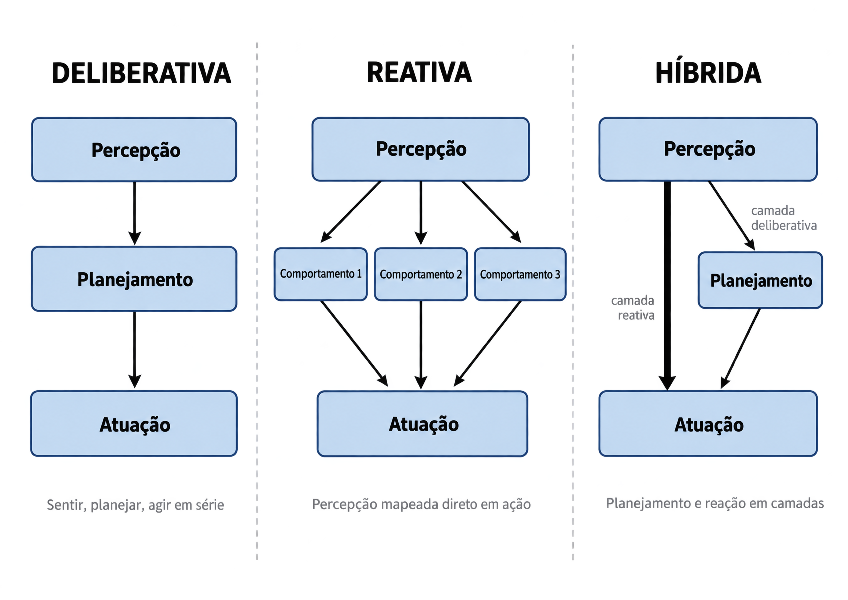
\includegraphics[width=0.8\textwidth]{figuras/fig_arquiteturas_roboticas.pdf}
    \caption{Paradigmas arquiteturais em robótica: as três colunas empregam as mesmas
    caixas --- percepção, planejamento e atuação ---, variando apenas como se conectam.
%% Corrigido em 14/11/2026: a legenda dizia que a camada reativa "alcanca a
%% atuacao sem passar pelo planejamento" e que esse e o paradigma da proposta. Nao e o
%% da implementacao: a camada reativa envia METAS ao Nav2, que continua planejando e
%% controlando, e permanece o unico produtor de /cmd_vel. O que a reacao contorna e a
%% DECISAO da patrulha sobre para onde ir, nao o planejamento do movimento.
    A via rápida em traço grosso na coluna híbrida é a camada reativa, que no esquema
    canônico alcança a atuação sem passar pelo planejamento. A arquitetura proposta no
    Capítulo~\ref{cap:proposta} segue esse paradigma em um sentido mais restrito, que
    convém fixar desde já: a camada reativa \emph{preempta a decisão} da patrulha sobre
    qual meta perseguir, mas não contorna o planejamento nem o controle de movimento ---
    ela envia metas ao Nav2, que permanece o único produtor de comandos de velocidade.}
    \legend{Fonte: Adaptado de \citeonline{Kortenkamp2016} e
    \citeonline{Brugali2009ComponentI}.}
    \label{fig:arquiteturas_roboticas}
\end{figure}


\subsection{Introdução ao ROS e ROS2}

O Robot Operating System (ROS) surgiu como uma resposta aos desafios arquiteturais dos sistemas robóticos, oferecendo um framework flexível e ferramentas para o desenvolvimento de software robótico \cite{Quigley2009}.

\subsubsection{Visão Geral do ROS}

Contrariamente ao que o nome sugere, o ROS não é um sistema operacional no sentido tradicional, mas sim um middleware que fornece serviços de comunicação, abstração de hardware, gerenciamento de pacotes e ferramentas para desenvolvimento de aplicações robóticas \cite{Quigley2009, Joseph2018}.

Os principais objetivos do ROS incluem abstração de hardware, computação distribuída, reutilização de código, ferramentas para testes e depuração, e criação de um ecossistema de software para a comunidade robótica \cite{Quigley2009}.

\subsubsection{Evolução para ROS2}

Apesar do sucesso do ROS, limitações em seu design original levaram ao desenvolvimento do ROS2, uma reimplementação completa que visa abordar essas limitações e adaptar-se às novas tendências em robótica \cite{Macenski2022}.

As motivações declaradas para o desenvolvimento do ROS2
\cite{Macenski2022, ROS2Design2024} dividem-se entre garantias que o ROS original não
dava e contextos que ele não atendia. Do primeiro grupo são o suporte a tempo real, os
mecanismos de segurança de autenticação, autorização e criptografia, a robustez em redes
não ideais e a confiabilidade exigida por aplicação industrial. Do segundo, a otimização
para sistemas embarcados de recurso limitado e o suporte nativo à coordenação de
múltiplos robôs. A primeira dessas garantias é a que importa ao Capítulo~\ref{cap:proposta},
e a Seção~\ref{sec:prop-relogios} mostra que tê-la disponível não equivale a tê-la
usada corretamente.

\subsection{Arquitetura e Componentes do ROS/ROS2}

Tanto o ROS quanto o ROS2 seguem uma arquitetura baseada em componentes, com alguns conceitos fundamentais compartilhados, embora com implementações diferentes \cite{Quigley2009, Macenski2022}.

\subsubsection{Conceitos Fundamentais}

\paragraph{Nós}

Os nós são os processos computacionais básicos no ROS/ROS2, responsáveis por realizar computações específicas \cite{Quigley2009, Joseph2018}. Em ROS, os nós são processos independentes que se comunicam através do ROS Master. Em ROS2, os nós podem ser processos independentes ou componentes dentro de um mesmo processo, com comunicação gerenciada pelo middleware DDS \cite{Macenski2022}.

\paragraph{Tópicos}

Os tópicos são canais de comunicação unidirecional que seguem o padrão publicador/assinante \cite{Quigley2009, Joseph2018}. Um nó publica mensagens em um tópico, e qualquer nó interessado pode se inscrever para receber essas mensagens. A comunicação via tópicos é assíncrona e desacoplada, adequada para transmissão contínua de dados como leituras de sensores ou estados do robô \cite{Macenski2022}.

\paragraph{Serviços e Ações}

Os serviços seguem o padrão cliente/servidor, onde um nó faz uma solicitação a outro e espera por uma resposta \cite{Quigley2009, Joseph2018}. São síncronos e adequados para operações discretas que requerem uma resposta.

As ações são uma extensão dos serviços para operações de longa duração, consistindo em uma meta, feedback durante a execução e um resultado final \cite{Joseph2018, Macenski2022}. São adequadas para tarefas como navegação ou manipulação de objetos.

\paragraph{Parâmetros e Bags}

Os parâmetros são valores de configuração que podem ser acessados e modificados pelos nós \cite{Quigley2009, Joseph2018}. Em ROS, são gerenciados pelo Parameter Server; em ROS2, pelos próprios nós.

Os bags são um formato de arquivo para armazenar e reproduzir mensagens ROS/ROS2, úteis para gravar dados durante a execução e reproduzi-los posteriormente para análise ou teste \cite{Quigley2009, Joseph2018}.

\subsubsection{Middleware e Comunicação}

Uma das principais diferenças entre ROS e ROS2 está na camada de middleware que gerencia a comunicação entre os componentes do sistema \cite{Macenski2022, ROS2Design2024}. A \autoref{fig:ros_vs_ros2} contrasta as duas arquiteturas de descoberta, separando o que é registro do que é tráfego de dados.

\paragraph{ROS Master vs. DDS}
\begin{figure}[h]
    \centering
%% Figura refeita em 14/11/2026. Na versao anterior o "Middleware DDS" aparecia como
%% hub central do painel ROS2, na mesma posicao e topologia do ROS Master a esquerda --
%% de modo que os dois paineis mostravam a MESMA arquitetura com nomes diferentes no
%% meio, apagando justamente a diferenca que a secao descreve. No painel ROS, todas as
%% ligacoes passavam pelo Master, reproduzindo o equivoco de que os dados trafegam por
%% ele. A fonte tambem nao citava nada ("documentacao oficial", sem referencia).
    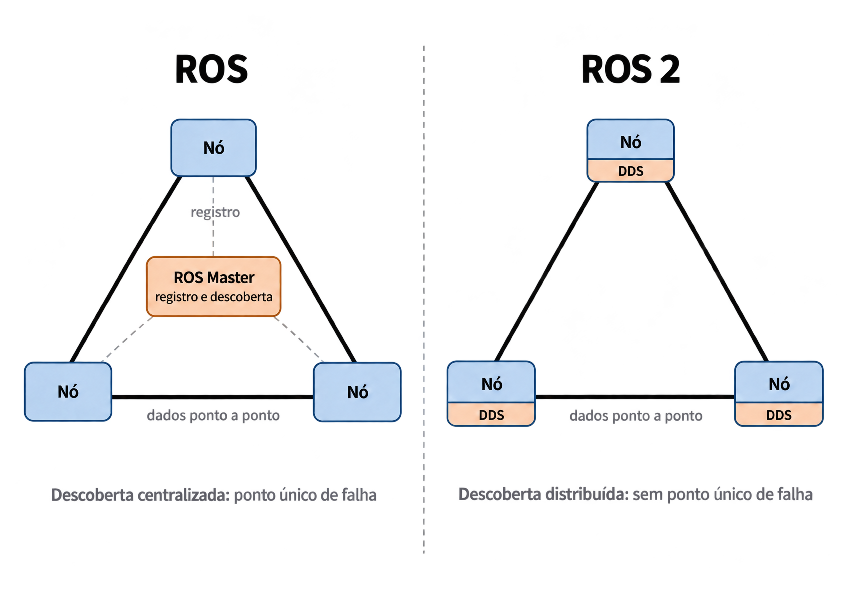
\includegraphics[width=0.8\textwidth]{figuras/fig_ros_vs_ros2.pdf}
    \caption{Arquiteturas de descoberta no ROS e no ROS~2, com os nós nas mesmas
    posições nos dois painéis. À esquerda, o registro (tracejado) é centralizado no ROS
    Master, enquanto os dados (linha cheia) trafegam ponto a ponto. À direita não há
    elemento central: o DDS reside dentro de cada nó e a descoberta é distribuída.}
    \legend{Fonte: Elaborada pelo autor com base em \citeonline{Macenski2022} e na
    documentação de projeto do ROS~2 \cite{ROS2Design2024}.}
    \label{fig:ros_vs_ros2}
\end{figure}

%% Precisado em 14/11/2026, junto com a figura: dizer que "a comunicacao e gerenciada
%% pelo ROS Master" induz a ideia de que os dados trafegam por ele, o que a figura nova
%% desmente explicitamente ao separar registro (tracejado) de dados (linha cheia).
No ROS original, é a \emph{descoberta} entre nós que é gerenciada pelo ROS Master, um serviço centralizado que mantém o registro de todos os nós, tópicos e serviços ativos \cite{Quigley2009, Joseph2018}. Concluída a negociação, os nós trocam mensagens diretamente entre si, ponto a ponto, sem que os dados passem pelo Master. Esta centralização da descoberta simplifica a implementação, mas introduz um ponto único de falha: sem o Master, nenhum nó novo encontra os demais.

O ROS2 substitui o ROS Master por uma arquitetura baseada em DDS (Data Distribution Service), um padrão aberto para comunicação publicador/assinante em sistemas distribuídos \cite{Macenski2022, ROS2Design2024}. O DDS oferece recursos avançados como descoberta distribuída, qualidade de serviço (QoS), segurança, persistência e filtragem de conteúdo.

\paragraph{Modelo de Computação}

No ROS original, cada nó é tipicamente um processo independente \cite{Quigley2009, Joseph2018}. O ROS2 introduz o conceito de composição de nós, permitindo que múltiplos nós sejam executados dentro do mesmo processo \cite{Macenski2022, ROS2Design2024}, reduzindo a sobrecarga de comunicação e permitindo compartilhamento mais eficiente de recursos.

Os executores em ROS2 gerenciam a execução de callbacks associados a tópicos, serviços, ações e timers, com diferentes tipos disponíveis (SingleThreadedExecutor, MultiThreadedExecutor, StaticSingleThreadedExecutor) para diferentes necessidades \cite{Macenski2022, ROS2Design2024}.

\subsection{Simulação e Validação}

A simulação é essencial no desenvolvimento de sistemas robóticos, permitindo testar algoritmos em ambientes virtuais antes da implementação em hardware real \cite{Siegwart2011}.

\subsubsection{Simuladores Integrados}

O ROS/ROS2 integra-se com diversos simuladores \cite{Joseph2018, Macenski2022}. O
\textbf{Gazebo} foi desenvolvido especificamente para robótica e oferece simulação de
física, de sensores, ambientes personalizáveis e extensibilidade por \textit{plugins}; é
o usado nesta tese. Webots, CoppeliaSim (V-REP), CARLA, voltado a veículos autônomos, e
Isaac Sim, da NVIDIA, também se integram ao ROS/ROS2.

\subsubsection{Ferramentas de Simulação e Teste}

O ROS/ROS2 oferece ferramentas como URDF/XACRO para descrição de robôs, RViz para visualização 3D, e rqt para interfaces gráficas \cite{Joseph2018, Macenski2022}. Para validação, integra-se com frameworks de teste unitário (GTest, pytest) e oferece ferramentas para testes de integração e integração contínua \cite{Joseph2018, Macenski2022}.

%% Subsecao NOVA em 15/11/2026, construida em torno do paragrafo que antes era a cauda
%% orfa de "Tendencias e Desenvolvimentos Futuros". O determinismo de temporizacao e a
%% unica materia desta secao que reaparece nos capitulos posteriores (15 ocorrencias de
%% tempo simulado / relogio de parede neles, contra 2 aqui), e e a fundamentacao do
%% defeito relatado na Secao 6.13. Merecia subsecao, nao um paragrafo pendurado no fim.
%% Removidas no mesmo passo as subsecoes de Integracao de Sensores e Atuadores,
%% Desenvolvimento de Aplicacoes, Aplicacoes e Casos de Uso e Tendencias: zero
%% ocorrencias de catkin, ament_cmake, setuptools, rosbag, rostopic, rosparam, tf,
%% manipulador, micro-ROS e computacao em nuvem em QUALQUER outro capitulo da tese.
\subsection{Tempo Simulado e Determinismo de Temporização}
\label{sec:fund-relogios}

Em simulação, o \ac{ROS}~2 permite que todos os nós compartilhem uma base de tempo
publicada pelo simulador, em vez do relógio do sistema operacional. Habilitado o
parâmetro correspondente, os temporizadores de cada nó passam a ser disparados por esse
tempo \emph{simulado}, de sorte que uma pausa do simulador pausa também o agendamento, e
uma simulação que corra mais devagar ou mais depressa que o tempo real não altera o
intervalo \emph{percebido} entre dois disparos \cite{Macenski2022}. É essa propriedade que
torna um experimento em simulação repetível, independentemente da carga da máquina em que
roda.

A propriedade, porém, vale para o mecanismo de agendamento, não para o código agendado.
Um temporizador pode ser disparado em tempo simulado enquanto a função que ele chama
consulta, internamente, o relógio de parede do processo --- e nada na interface sinaliza a
divergência, porque as duas leituras têm o mesmo tipo e a mesma aparência. Se essa função
compara dois instantes para decidir se um intervalo transcorreu, ela passa a medir numa
base de tempo e a ser chamada em outra, e o intervalo efetivo deixa de ser o
especificado. A Seção~\ref{sec:prop-relogios} descreve a ocorrência desse padrão na
implementação avaliada neste trabalho, e a Seção~\ref{sec:res-verificacao-relogio} mede a sua
consequência sobre os desfechos.